\chapter{Physics Analysis}

The analysis here presented corresponds to the search for rare decays of $H \rightarrow \Upsilon + \gamma$, where the $\Upsilon$ might appear in the states $1S$, $2S$ or $3S$, and shall decay to a pair of muons (from here on, called dimuon system) and the $\gamma$ will be identified as a offline reconstructed photon. The decay to the dimuon channel offers a very efficient triggering for this process, characteristic of CMS. The analogous process of the $Z$ boson decays to the same channel is also studied, as a benchmark for the Higgs decay.

The main process contributing to the accessible phase space of these decays are described in Figure~\ref{analysis_process_diagram}, in which the different process are represented in a diagram for the reconstructed invariant masses of the muon-muon-photon system ($\mu\mu\gamma$ - horizontal axis) and the muon-muon system ($\mu\mu$ - vertical axis). The vicinity of the $H/Z$ mass and $\Upsilon$ mass regions are represented in the midpoint for each axis. The backgrounds can be divided in \textbf{Resonant} and \textbf{Non-Resonant} backgrounds. The Non-Resonant might come from two sources, a Full Combinatorial background is composed by the combination of two non-correlated muons with a photon in the final state of the event. This is expected to be spread all over the phase space and in the diagram, it is represented by the color blue. The $\Upsilon+ \gamma$ Combinatorial background is a combination of two correlated muons (e.g.: the decay of a $\Upsilon$ to a dimuon muon system) combined with a photon from a secondary process (e.g.: Multiple Particle Interaction - MPI, pileup, a jet mis-identified as a photon). This should be concentrated in the region around the $\Upsilon(1S, 2S, 3S)$ and it is represented by the gray region.

% analysis process 
\begin{figure}[htbp]
    \centering
    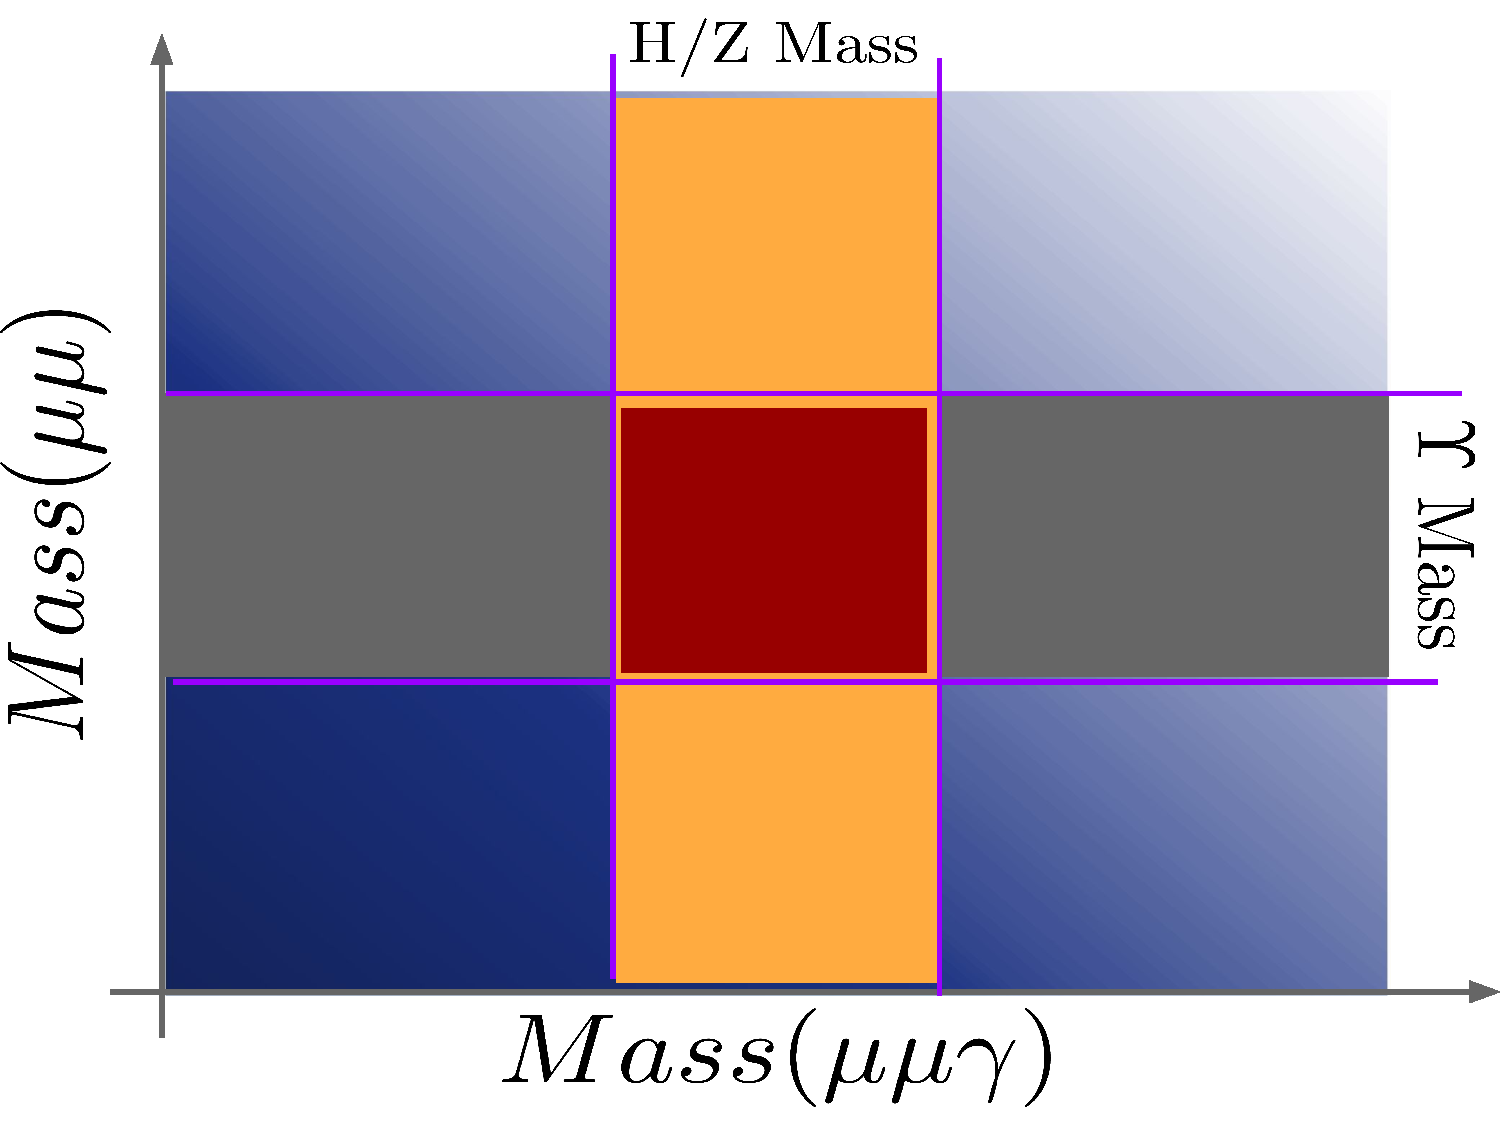
\includegraphics[width=0.6\textwidth]{figures_and_tables/analysis_process.pdf}
    \caption{A diagram for the reconstructed invariant mass of the $\mu\mu\gamma$ final state. The blue and gray regions represent the Full Combinatorial and $\Upsilon + \gamma$ Combinatorial contributions, respectively, while the yellow and red regions represent the Resonant background and the signal region.}
    \label{analysis_process_diagram}
\end{figure}

The Resonant background is composed by the processes where the boson (Higgs or Z) decays to a $\mu\mu\gamma$ final state without going trough the the intermediate meson state. For the Z decays, this background is modeled based on a Drell-Yan to dimuon decays, with a final state radiated (FSR) photon ($Z \rightarrow \mu\mu\gamma_{FSR}$), while for the Higgs decay, a  Higgs Dalitz decay ($H \rightarrow \mu\mu\gamma$) is used. The Resonant background (also called Peaking Background) is represented in the diagram by the region in yellow. The Signal is represented by the red region on the diagram.

Around these representations, the a 2-dimensional model of the reconstructed invariant masses ($m_{\mu\mu\gamma}$ and $m_{\mu\mu}$) is constructed for each contributing process and tested against the collected data by the experiment, by means of a unbinned maximum likelihood fit. No significant excess above the background-only model is observed and a upper limit of the signal branch fraction is extracted. The following sections describes the data and simulated samples used in this analysis, the event selection applied in order to enhance the signal to background ratio and the process to construct the statistical models used in the upper limits extraction.
